\documentclass[format=acmtog]{acmart}
% Packages
%\usepackage{mathtools}
%\usepackage{amssymb}
%\usepackage{fixltx2e}
%\usepackage{ntheorem}
%\usepackage{float}
%\usepackage{xr}
%\usepackage{array}
%\usepackage[justification=centering]{caption}
%\usepackage{pifont}
%\usepackage{verbatim}
%\usepackage[english]{babel}
%\usepackage{wrapfig}
%\usepackage{capt-of}
%\usepackage{color}
%\usepackage{pdftricks}
%\usepackage{etex}
%\usepackage[version=0.96]{pgf}
%\usepackage{proof}
%\usepackage{latexsym}
%\usepackage{amsfonts}
%\usepackage{stackrel}
%\usepackage{cases}
\usepackage{subcaption}
\usepackage{pgfplots}
\captionsetup{compatibility=false}%\usepackage{subfig}
\usepackage{changepage}
\usepackage{amssymb}
\usepackage{amsmath}
%\usepackage{amsthm}
\usepackage{graphicx}
\usepackage{url}
\usepackage{multirow}
\usepackage{enumitem}
\usepackage{ifthen,stackengine}
\usepackage{tikz}
\usepackage{cases}
\usepackage{mathtools}
\usetikzlibrary{patterns,intersections,plotmarks,calc,arrows,shapes,snakes,automata,backgrounds,petri,positioning,fit}

% beamer presentation
\newcommand{\keyword}[1]{\textcolor{bordeau}{#1}}


\definecolor{ltgreen}{RGB}{180, 202, 72}
\definecolor{mdgreen}{RGB}{138, 181, 78}
\definecolor{dkgreen}{RGB}{0, 153, 0}
\definecolor{dgreen}{rgb}{.2,.7,.2}
% theorems

% specific environment
%\newenvironment{comment}{\vspace*{0.5cm} \noindent \underline{Note :} }{\vspace*{0.5cm}}
%\newenvironment{proof}[1]{\noindent\textbf{Proof#1:}}{\hspace*{0.25cm}$\Box$ \vspace*{0.25cm}}
%\newenvironment{proposition}{\begin{beamerboxesrounded}[shadow=true]{Proposition}}{\end{beamerboxesrounded}}

% maths
\newcommand{\simu}[1]{\sqsubseteq_{#1}}
\newcommand{\pmax}[1]{\textbf{max} \ #1}
\newcommand{\pmin}[1]{\textbf{min} \ #1}
\newcommand{\ppmax}[2]{\textbf{max}_{#2} \ #1}
\newcommand{\ppmin}[2]{\textbf{min}_{#2} \ #1}
\newcommand{\false}{\textnormal{\textit{false}}}
\newcommand{\true}{\textnormal{\textit{true}}}
\newcommand{\func}[2]{#1(#2)}
% sets
\newcommand{\deltami}{\delta_{\min}}                 %non negative integer values
\newcommand{\deltama}{\delta_{\max}(\alpha)}                 %non negative integer values
\newcommand{\deltamax}{\delta_{\max}}                 %non negative integer values
\newcommand{\deltamin}{\delta_{\min}}                 %non negative integer values
\newcommand{\integerpoz}{\mathbb Z_{\ge 0}}                 %non negative integer values
\newcommand{\integerpos}{\mathbb Z_{> 0}}                 %non negative integer values
\newcommand{\integer}{\mathbb{Z}}                 % integer values
\newcommand{\real}{\mathbb{R}}                    % real numbers
\newcommand{\realpos}{\mathbb R_{> 0}}               % non-negative real numbers
\newcommand{\realposz}{\mathbb R_{\ge 0}}               % non-negative real numbers
\newcommand{\realpoz}{\mathbb R_{\ge 0}}               % non-negative real numbers
\newcommand{\ii}{\imath}
\newcommand{\jj}{\jmath}
% time
\newcommand{\hmnb}[1]{h_{\min}(#1)}
\newcommand{\hmxb}[1]{h_{\max}(#1)}
\newcommand{\hmn}{h_{\min}(\alpha)}
\newcommand{\hmx}{h_{\max}(\alpha)}
\newcommand{\timeval}{\mathbb{T}}                 % set of time values
\newcommand{\tc}{\textrm{tc }}       % lower bound of tc
\newcommand{\lbtc}{\mathtt{l}}       % lower bound of tc
\newcommand{\ubtc}{\mathtt{u}}       % upper bound of tc
\newcommand{\Q}{\mathrm{Q}}       % urgency type lazy
%\newcommand{\G}{\mathcal{G}}       % urgency type lazy
\newcommand{\Loc}{\mathcal{L}}       % urgency type lazy
\newcommand{\lazy}{\mathrm{l}}       % urgency type lazy
\newcommand{\delayable}{\mathrm{d}}  % urgency type delayable
\newcommand{\eager}{\mathrm{e}}      % urgency type eager
\newcommand{\I}{\mathcal{I}}      % urgency type eager
\newcommand{\reset}{\textnormal{\textsf{reset}}}  % reset a list of clocks
\newcommand{\clks}{\textnormal{\textsf{X}}}       % set of clocks
\newcommand{\val}{v}                              % valuation of the clocks
\newcommand{\valg}{\bar{v}}                              % valuation of the clocks
\newcommand{\valgp}{\bar{v'}}                              % valuation of the clocks
\newcommand{\Val}{\mathcal{V}}                              % valuation of the clocks
\newcommand{\vals}[1]{\textnormal{\textsf{V(}}#1\textnormal{\textsf{)}}}% set of valuations
\newcommand{\urg}{\textnormal{\textit{urg}}}      % urgency predicate: true iff the guard is urgent
%\newcommand{\q}{\tsf{q}}      % urgency predicate: true iff the guard is urgent
\newcommand{\q}{q}      % urgency predicate: true iff the guard is urgent
\newcommand{\x}{\tsf{x}}      % urgency predicate: true iff the guard is urgent
\newcommand{\urgb}{\tsf{urg}}      % urgency predicate: true iff the guard is urgent
\newcommand{\confl}{\mathit{conf}}      % urgency predicate: true iff the guard is urgent
\newcommand{\obs}{\tsf{obs}}      % urgency predicate: true iff the guard is urgent
%\newcommand{\guard}{\textnormal{\textsf{guard}}}  % 
\newcommand{\wait}{\textnormal{\textsf{wait}}}
\newcommand{\untimed}{\textnormal{\textsf{u}}}    % untimed transitions
\newcommand{\timed}{\textnormal{\textsf{t}}}      % timed transitions
\newcommand{\tpc}[1]{\mathit{tpc}_{#1}}
\newcommand{\tpcb}{\textnormal{\mathit{tpc}}}
\newcommand{\hastpc}{\textnormal{\texttt{hastpc}}}
\newcommand{\enables}{\textnormal{\texttt{ enables }}}
\newcommand{\nenables}{\textnormal{\texttt{$\neg$enables }}}

% ideal model
\newcommand{\relt}[1]{\stackrel{#1}{\longrightarrow}} % transition relationship
\newcommand{\locs}{\textnormal{\textsf{Q}}}       % set of control locations
\newcommand{\p}[1]{\mathrm{part}(#1)}       % set of control locations
\newcommand{\cp}{B=\gamma(B_1,\cdots,B_n)}  % composition
%\newcommand{\guards}[1]{\textnormal{\textsf{G(}}#1\textnormal{\textsf{)}}} % set of guards over a set of clocks
\newcommand{\TC}[1]{\textnormal{\textsf{TC(}}#1\textnormal{\textsf{)}}} % set of guards over a set of clocks
\newcommand{\actions}{\textnormal{\textsf{A}}}    % set of actions
\newcommand{\states}{\textnormal{\textsf{S}}}     % set of states

% physical model
\newcommand{\etf}{\varphi}                        % execution time function
\newcommand{\instanceof}{\triangleleft}           % instance of
\newcommand{\waitloc}[1]{wait_{#1}}               % waiting control location for the completion of a given action
\newcommand{\complete}[1]{end_{#1}}               % completion action for a given action
\newcommand{\etclk}[1]{x_{#1}}                    % clock for counting the execution time of a given action


% implementation
\newcommand{\interactions}{\gamma}                % set of interactions
\newcommand{\enabledinteractions}[1]{\gamma_{#1}} % set of enabled interactions for a given {state}
\newcommand{\nextactivation}[2]{\textnormal{\textsf{next}}_{#2}(#1)}    % next activation
\newcommand{\nextdeadline}[2]{\textnormal{\textsf{deadline}}_{#2}(#1)}    % next deadline
\newcommand{\nexta}[1]{\mathrm{next(#1)}}
\newcommand{\deadline}[1]{\mathrm{deadline(#1)}}
% urgency
\newcommand{\urgency}[1]{\textcolor{red}{#1}}
\newcommand{\good}[1]{\textcolor{dgreen}{#1}}
% safe
\newcommand{\safe}{\textnormal{\texttt{safe}}}
%send receive
\newcommand{\bsr}[1]{B_{#1}^{SR}}
\newcommand{\ysr}{\gamma^{SR}}
\newcommand{\csr}{B^{SR}}

% thank you slide
\newcommand{\thankyou}%
{
    \frame{%

      \textbf{\Huge Thank You!}%
      \vspace{1cm}
      \begin{figure}
        
\includegraphics[scale=1]{../images/question.pdf}  \\
      \end{figure}
      \vspace{1cm}
      \insertauthor \\
      \vspace{0.60cm}
      
    }%
}

\newcommand{\barrow}{\item[\color{red}\ding{227}]}
\newcommand{\yes}{\textcolor{dkgreen}{\ding{58}}} % green +
\newcommand{\byes}{\scalebox{3}{\textcolor{dkgreen}{\ding{58}}}} % green +
\newcommand{\no}{\textcolor{dkorange}{\ding{54}}} % red X
\newcommand{\notsure}{\textcolor{mdgrey}{\textbf{???}}} % grey ???
\newcommand{\neutral}{\textcolor{mdgrey}{$\bm{\sim}$}} % grey ~



\newcommand{\ie}{i.\,e.\xspace}
\newcommand{\eg}{e.\,g.\xspace}
\newcommand{\warning}[1]{
\includegraphics[width=.3cm]{../images/warning.pdf}~~#1}
\newcommand{\warnings}{
\includegraphics[scale=.4]{../images/warning.pdf}}
%fonts
\newcommand{\transit}[1]{\xrightarrow{#1}}
\newcommand{\transitb}[1]{\stackrel{#1}{\leadsto}}
\newcommand{\transitbp}[1]{\stackrel{#1}{\leadsto}_{\pi\gamma}}
\newcommand{\bv}{\textnormal{\textbf{v}}}
\newcommand{\inv}{\mathit{tpc}}
%\newcommand{\inv}{\textnormal{tpc}}
%\newcommand{\C}{\mathcal{C}}
\newcommand{\Y}{\mathcal{Y}}
\newcommand{\X}{\mathcal{X}}
\newcommand{\R}{\mathcal{R}}
\newcommand{\T}{\mathcal{T}}
\newcommand{\A}{\mathcal{A}}
\newcommand{\tsf}[1]{\textnormal{\textsf{#1}}}
\newcommand{\tsfb}[3]{\textnormal{\textsf{#1}\textsubscript{#2}\textsuperscript{#3}}}
\newcommand{\tib}[1]{\textbf{\textit{#1}}}
\newcommand{\tb}[1]{\textbf{#1}}
\newcommand{\ti}[1]{\textit{#1}}
\newcommand{\tcal}[1]{\mathcal{#1}}
\newcommand{\tr}[1]{TR_{#1}}
\newcommand{\cn}{\textit{B}}
\newcommand{\msucc}{\textnormal{\textsf{succ}}}
\newcommand{\tsucc}{\textnormal{\textsf{time-succ}}}
\newcommand{\dsucc}{\textnormal{\textsf{disc-succ}}}
\newcommand{\close}{\textnormal{\textsf{norm}}}
\newcommand{\reach}{\textit{Reach}}
\newcommand{\ic}{\textit{CI}}
\newcommand{\iim}{\textit{II}}

\newcommand{\guard}[2]{\mathit{guard}(#1,#2)}
\newcommand{\ex}{\sigma}
\newcommand{\reachable}{\tsf{Reach}}
\newcommand{\locations}[1]{\mathcal{L}_{#1}}
\newcommand{\plan}[1]{\mathit{\mathbf{plan}}(#1)}
\newcommand{\plana}{\textnormal{\tb{plan}}}
\newcommand{\enabled}{\mathit{Enabled}}
\newcommand{\disabled}{\mathit{Disabled}}
\newcommand{\enabledfrom}{\mathit{Enabled}^{{\scriptscriptstyle \nearrow^{\delta}}}}
\newcommand{\enabledfrombis}[1]{\mathit{Enabled}^{{\scriptscriptstyle \nearrow^{#1}}}}
\newcommand{\enabledfromz}{\mathit{Enabled}^{{\scriptscriptstyle \nearrow^0}}}
\newcommand{\enabledfromd}{\mathit{Enabled}^{{\scriptscriptstyle \nearrow^{[0,\deltama]}}}}
\newcommand{\enabledfromdi}{\mathit{Enabled}^{{\scriptscriptstyle \nearrow^{[0,h(\alpha)]}}}}
\newcommand{\zoneplan}{\swarrow^{\deltamax}_{\deltamin}}
\newcommand{\zonep}[1]{\swarrow^{#1}}
\newcommand{\at}[1]{\tsf{at}(#1)}
\newcommand{\backward}{\swarrow}
\newcommand{\backwardd}{\swarrow^{\deltama}}
\newcommand{\historyineq}{\mathcal{E}}
\newcommand{\rise}{\uparrow}
\newcommand{\fall}{\downarrow}
\newcommand{\backwarduntil}[1]{_{#1}\makebox[2.1ex][r]{$\backward$}}
\newcommand{\interactioninvariants}[1]{\mathcal{II}}
\definecolor{aqua}{rgb}{0.5, 1.0, 0.83}
\definecolor{aqua2}{rgb}{0.5, 1.0, 0.83}
%maths
\newenvironment{rrcases}
  {\left.\begin{numcases}}
  {\end{numcases}\right\rbrace}

\newcommand{\LeftEqNo}{\let\veqno\@@leqno}
\newcommand{\sched}{\mathit{schedule}}
\newcommand{\loc}{\ell}
\newcommand{\locg}{\bar{\ell}}
\newcommand{\locgp}{\bar{\ell'}}
\newcommand{\equi}{\Leftrightarrow}
\newcommand{\lto}{\longrightarrow}
\newcommand{\llto}[1]{\overset{#1}{\leadsto}}
\newcommand{\shiftpoints}{4pt}


\newcommand{\ta}{(\Loc,\loc_0,\A,\T,\X,\inv)}
\newcommand{\tab}[1]{(\Loc_{#1},\loc_0^{#1},\A_{#1},T_{#1},\X_{#1},\tpc_{#1})}
\newcommand{\lts}{(\Q,\A\cup\realpos,\to)}
\newcommand{\ltsg}{(\Q_g,\gamma\cup\realpos,\lto)}
\newcommand{\squig}{{\scriptstyle\sim\mkern-3.9mu}}
\newcommand{\lsquigend}{{\lhd\mkern-3mu}}
\newcommand{\rsquigend}{{\scriptstyle\rule{.1ex}{0ex}>}}
\newcounter{sqindex}
\newcommand\squigs[1]{
    \setcounter{sqindex}{0}
      \whiledo {\value{sqindex}< #1}{\addtocounter{sqindex}{1}\squig}
    }
\newcommand{\tranbp}[2]{
  \mathbin{\stackon[2pt]{\squigs{#2}\rsquigend}{\scriptstyle{#1\,}}}_{\gamma}
      }

\newcommand{\Depth}{1}
\newcommand{\Height}{1.75}
\newcommand{\Width}{0.5}

\newcommand{\backhtxt}{\swarrow^{\hmx}_{\hmn}}
\newcommand{\backhtxtb}{\swarrow^{\hmx}_{\hmn}}
\newcommand{\backh}{\swarrow^{\hmx}_{\hmn}g(x)\Leftrightarrow\exists\delta\in[\hmn,\hmx].g(x+\delta),}

\newcommand{\plntxt}[1]{\mathit{Plannable(#1)}}
\newcommand{\pln}[1]{\mathit{Plannable(#1)}=\bigvee_{\loc\in\Loc_{#1}}
\at{\loc}\wedge\backhtxt(\bigwedge_{a_i\in#1} \guard{a_i}{\loc_i})}

\newcommand{\plnIntxt}[2]{\mathit{Plannable(#1,#2)}}
\newcommand{\plnIn}[2]{\mathit{Plannable(#1,#2)}=\bigvee_{\loc\in\Loc_{#1}}
\at{\loc}\wedge\bigwedge_{a_i\in#1} \Big(\guard{a_i}{\loc_i}+#2\Big)}


\newcommand{\stat}{%
\smash{\raisebox{.5\dimexpr3\baselineskip+4\itemsep+2\parskip}{$\left.\rule{0pt}{.5\dimexpr4\baselineskip+3\itemsep+3\parskip}\right\}$\ \parbox{5.5cm}{dynamically checked during execution}}}
}
\newcommand{\dyn}{%
\smash{\raisebox{.5\dimexpr3\baselineskip+4\itemsep+2\parskip}{$\left.\rule{0pt}{.5\dimexpr4\baselineskip+3\itemsep+3\parskip}\right\}$\ \parbox{5.5cm}{dynamically checked during execution}}}
}


\newlength{\mywidth}                          
\newcommand\bigfrown[2][\textstyle]{\ensuremath{%
  \array[b]{c}\text{\resizebox{\mywidth}{.7ex}{$#1\frown$}}\\[-1.3ex]#1#2\endarray}}
 \settowidth{\mywidth}{$\enabledfromd(\alpha)$}

 
 \makeatletter
\def\namedlabel#1#2{\begingroup
  \mbox{\hspace{1cm}}#2%
    \def\@currentlabel{#2}%
    \phantomsection\label{#1}\endgroup
}
\makeatother

\makeatletter
\newcommand{\mytag}[2]{%
 \text{#1}%
  \@bsphack
    \protected@write\@auxout{}%
   {\string\newlabel{#2}{{#1}{\thepage}}}%
  \@esphack
}          
\makeatother

\newtheorem{property}{Property}
\stackMath


% Metadata Information
\acmJournal{TOG}

\tikzset{                                 
    connect/.style args={(#1) to (#2) over (#3) by #4}{
    insert path={                         
      let                             
      \p1=($(#1)-(#3)$),            
      \n1={veclen(\x1,\y1)},        
      \n2={atan2(\y1,\x1)},         
      \n3={abs(#4)},                
      \n4={#4>0 ?180:-180}          
              in                            
              (#1) -- ($(#1)!\n1-\n3!(#3)$) 
              arc (\n2:\n2+\n4:\n3) -- (#2) 
      }                                     
    }                                       
}        
\begin{document}

\title{TBA}
\author{Mahieddine Dellabani}
\affiliation{%
    \institution{University Grenoble Alpes, VERIMAG}
    \city{Grenoble}
    \country{France}
  }
\author{Jacques Combaz}
\affiliation{%
    \institution{University Grenoble Alpes, VERIMAG}
    \city{Grenoble}
    \country{France}
  }
\author{Mohamed Foughal}
\affiliation{%
    \institution{LAAS}
    \city{Toulouse}
    \country{France}
  }
\author{Saddek Bensalem}
\affiliation{%
    \institution{University Grenoble Alpes, VERIMAG}
    \city{Grenoble}
    \country{France}
  }



\renewcommand\shortauthors{Dellabani, Combaz, Foughal et al}



\begin{abstract}
Design, implementation and verification of distributed real-time systems is acknowledged to be a very hard task.
These type of systems are prone to different kind of delays, such as execution times of actions or communication delays implied by the distributed platform.
This increases considerably the complexity of coordinating the parallel activities of running components.
In order to ensure global consistency and timing constraints satisfaction, scheduling of such systems must cope with those delays, and propose and execution strategy to avoid execution failure. 
In this paper, we investigate a formal model for such systems as compositions of timed automata subject to multi-party interactions and we propose 
method aiming to overcome the communication delays problem through planning ahead interactions. Moreover, we propose different verification technics for checking dealock-freedom property for the proposed approach and hightlight the complexity of verifying this property.
\end{abstract}


\begin{CCSXML}
  <ccs2012>
  <concept>
  <concept_id>10003752.10003766</concept_id>
  <concept_desc>Theory of computation~Formal languages and automata theory</concept_desc>
  <concept_significance>500</concept_significance>
  </concept>
  <concept>
  <concept_id>10003752.10003790.10002990</concept_id>
  <concept_desc>Theory of computation~Logic and verification</concept_desc>
  <concept_significance>500</concept_significance>
  </concept>
  <concept>
  <concept_id>10010520.10010553</concept_id>
  <concept_desc>Computer systems organization~Embedded and cyber-physical systems</concept_desc>
  <concept_significance>500</concept_significance>
  </concept>
  </ccs2012>
\end{CCSXML}

\ccsdesc[500]{Theory of computation~Formal languages and automata theory}
\ccsdesc[500]{Theory of computation~Logic and verification}
\ccsdesc[500]{Computer systems organization~Embedded and cyber-physical systems}

\keywords{Distributed Real-Time Systems$\cdot$Timed Automata$\cdot$Compositional Verification}




\maketitle
\section{Introduction}

Nowadays, real-time systems are ubiquitous in several application domains, 
and such an emergence led to an increasing need of performance: resources, 
availability, concurrency...etc. This expansion initiate a shift from the
use of single processor based hardware platforms, to large sets 
of interconnected and distributed computing nodes, and even gave birth to
a new family of system known as \emph{Networked Embedded Systems}, and
that are intrinsically distributed.
Such evolution stems from an increase in complexity of real-time software 
embedded on such platforms (e.g. electronic control in avionics 
and automotive domains~\cite{Charette09}), and the need to integrate 
formerly isolated systems~\cite{Kopetz:2004:IAD:1032662.1034360} so that 
they can cooperate as well as share resources, improving functionality 
and reducing costs.

To deal with such complexity, the community of safety critical systems 
often restricts its scope to predictable systems, which are represented 
with domain specific models (e.g. periodic tasks, synchronous systems, 
time-deterministic systems) for which the range of possible executions 
is small enough to be easily analyzed, allowing the pre-computation 
of optimal control strategies.
\emph{Networked Embedded Systems} usually describes a set of real-time systems, 
distributed across platform(s) and interacting through a network. 
Because of their adaptive behavior, the standard practice when implementing 
such systems is not to rely on models for pre-computation but rather to design
systems dynamically adapting at runtime to the actual context of execution.
Such approaches do not offer any formal guarantee of timeliness.
The lack of a priori knowledge on system behavior leaves also little room for 
static optimization.

Model-based development is one promising approach in building distributed 
real-time system. First, an application model is designed, expressing 
abstraction of the timed system behavior. This abstraction is platform 
independent, meaning that it does not consider platform introduced delays 
or CPU speed, which allow to: \emph{(i)} model the system at early stages 
without any knowledge of the target platform, and \emph{(ii)} verify 
the obtained model against some safety properties (functional requirements).
Thereafter, the application source code, which represents the actual 
implementation of the system on a given platform, 
is automatically generated from the model. The big challenge becomes then 
how to verify the timing behavior of the implementation, since a lot of 
assumption drops such as atomic execution of action or timeless communication delays. 

\indent In this paper, we propose an extension of the work presented in (cite fm) 
consisting in a model-based approach aiming to mitigate the communication delays of 
distributed platforms. In this approach, systems consist of components represented 
as timed automata that may synchronize on particular actions to coordinate 
their activities. We contribute to this research field by proposing methods for 
scheduling interactions with bounded horizons aiming to reduce the impact of 
communication delays on systems execution.
We extend our previous work by defining lower bound horizons for planning interactions, 
which correspond to the platform communication delays.
In particular, \emph{(i)} we exetend the semantics of (cite fm) for \emph{planning} interactions with 
lower bound horizons, \emph{(ii)} we discuss different methodologies for checking deadlock 
freedom property for such models, and \emph{(iii)} highlight the key issues met during our reflection. 

The rest of the paper is organized as follows. In Section~\ref{sec2}, 
we provide a definition of timed automata with respect to multiparty interactions. 
In Section~\ref{sec3}, we discuss the existing gap between the application model and
its implementation. Then, we propose a formal semantics based on planning
interactions with bounded horizons aiming to shorten this gap.
Thereafter, we propose different verification approaches for checking deadlock
freedom property of the presented model (Section~\ref{sec4}). 

\section{Timed Systems and Properties}
\label{sec2}

In the framework of the present paper, components are timed automata
and systems are compositions of timed automata with respect to
multiparty interactions. The timed automata we use are essentially
the ones from~\cite{alur94}, however, slightly adapted to embrace a
uniform notation throughout the paper.

\begin{definition}[Component]
  \label{def:atom}
  A \emph{component} is a tuple
  $(\Loc, \loc_0, A, T, \X, \inv)$ where
  $\Loc$ is a finite set of \emph{locations}, $\loc_0 \in \Loc$ is an \emph{initial} location, $A$
  a finite set of \emph{actions}, $\X$ is a finite set of
  \emph{clocks}, $T \subseteq \Loc\times(A\times \tcal{C}
  \times 2^{\X})\times \Loc$ is a set of \emph{transitions} labeled with an action, a
  guard, and a set of clocks to be reset,
  and $\inv: \Loc\rightarrow\tcal{C}$ assigns a \emph{time
    progress condition}, $\tpc{\loc}$,
    to each location, where $\tcal{C}$ is the set of \emph{clock
  constraints} defined by the following grammar: 
  \begin{displaymath} 
  C := \true \mid x\sim\mathit{ct} \mid x - y \sim\mathit{ct} \mid C 
\wedge C\mid\false, 
\end{displaymath}
  with $x, y\in \X$, $\sim$ $\in\{<,\le,=,\ge,>\}$ and $\mathit{ct} \in
  \mathbb{R}_{\ge 0}$.
 Time progress conditions are restricted to conjunctions of
  constraints of the form $x \leq \mathit{ct}$.
\end{definition}

Throughout the paper, we consider that components are deterministic timed automata, that is, 
at a given location $\loc$ and for a given action $a$, there is at most one outgoing transition from $\loc$ labeled by $a$. 
Given a timed automaton $(\Loc, \loc_0, A, T, \X, \inv)$, we write $\loc \transit{a,g,r} \loc'$ 
if there exists a transition $\tau = \big(\loc,(a,g,r),\loc'\big) \in T$. 
We also write: 
\begin{displaymath}
  \guard{a}{\loc}=
  \begin{cases}
    g, &\text{ if } \exists\tau = \big(\loc,(a,g,r),\loc'\big) \in T\\
    \false, &\text{ otherwise }
  \end{cases}
\end{displaymath}
Let $\Val$ be the set of all clock valuation functions
$\val: \X\rightarrow \mathbb{R}_{\ge
  0}$. 
For a clock constraint $C$, $C(\val)$ is a boolean value corresponding to the evaluation of $C$ on
$\val$. For a valuation $v \in \Val$, $\val + \delta$ is the valuation satisfying
$(\val + \delta)(x) = \val(x) + \delta$, while for a subset of clocks $r$, $\val[r]$ 
is the valuation obtained from $\val$ by resetting clocks of $r$, i.e. 
$\val[r](x) = 0$ for $x\in r$, $\val[r](x) = \val(x)$ otherwise.
We also denote by $C+\delta$ the clock constraint $C$ shifted by $\delta$, i.e. such that $C(\val+\delta)$ iff $C(\val)$.
\begin{definition}[Semantics]
  \label{def:atom_sem}
  A component $B = (\Loc, \loc_0, A, T, \X, \inv)$ defines the labeled transition system (LTS) 
  $(\Q, A\cup\realpos, \rightarrow)$ where $\Q\subseteq\Loc\times\Val(\X)$ denotes the \emph{states} of $B$ 
  and  $\rightarrow\subseteq\Q\times(A\cup\realpos) \times
  Q$ denotes the set of transitions between states according to the rules:
    \begin{itemize}
    \item $(\loc,\val) \transit{a} (\loc',\val[r])$ if $\loc \transit{a,g,r} \loc'$, and $g(\val)$ is true (action step).
      %\wedge \tpc{\loc'}(\val[r])$ (action step).
      \item $(\loc,\val) \transit{\delta} (\loc,\val+\delta)$ if $\tpc{\loc}(\val+\delta)$ for $\delta\in\realpos$
      (time progress).
    \end{itemize}
\end{definition}
We define the predicate $\urg(\tpc{\loc})$ characterizing the urgency of a time progress condition
$\tpc{\loc}=\bigwedge\limits_{i=1}^m x_i\le ct_i$ at a state $(\loc,\val)$ as follows:
\begin{displaymath}
\urg(\tpc{\loc})=\bigvee_{i=1}^m (x_i=ct_i),
\end{displaymath}
An \emph{execution sequence} of $B$ from a state $(\loc,\val)$ is a path in the LTS starting at $(\loc,\val)$ and that 
alternates action steps and time steps (time progress), that is:
\begin{displaymath}
  (\loc_1,\val_1) \transit{\ex_1} \ldots \transit{\ex_i} (\loc_n,\val_n),n\in\integerpos,\sigma\in A\cup\realpos
\end{displaymath}
In this paper, we always assume components with \emph{well formed guards} meaning that transitions $\loc \transit{a,g,r} \loc'$ satisfy
$g(v)\Rightarrow\tpc{\loc}(\val)\wedge\tpc{\loc'}(\val[r])$ for any $v \in \Val$.
%Before defining the semantics of a component, we first fix some
%notation.
We say that a state $(\loc,\val)$ is \emph{reachable} if there is an execution sequence from the initial configuration $(\loc_0, \val_0)$ leading to 
$(\loc,\val)$, where $\val_0$ assigns $0$ to all clocks.
Notice that the set of reachable states is in general infinite, but it can be partitioned into a finite number of symbolic
states~\cite{tripakis98:thesis,bengtssonY03,henzinger94}.
A symbolic state is defined by a pair $(\loc,\zeta)$ where, 
$\loc$ is a location of $B$, and $\zeta$ is a zone, i.e. a set of clock valuations defined by a clock constraint (as defined in Definition~\ref{def:atom}).
Efficient algorithms for computing symbolic states and operations on zones are fully described in~\cite{bengtssonY03}.
Given symbolic states $\{ (\loc_j,\zeta_j) \}_{j \in J}$ of $B$, the predicate $\reach(B)$ characterizing the reachable states can be formulated as:
\begin{displaymath}
 \reach(B) = \bigvee_{j \in J} \at{\loc_j} \wedge \zeta_j, 
\end{displaymath}
where $\at{\loc_j}$ is true on states whose location is $\loc_j$, and clock constraint $\zeta_j$ is straightforwardly applied to clock valuation functions of states.

We also define the predicate $\enabled(a)$ characterizing states $(\loc, \val)$ at which an action $a$ is enabled, i.e. such that $(\loc,\val) \transit{a} (\loc',\val')$. It can be written:
\begin{displaymath}
\enabled(a) = \bigvee_{(\loc,a,g,r,\loc') \in T} \at{\loc}  \wedge \guard{a}{\loc}
\end{displaymath}


\begin{definition}[Deadlock]
  \label{def:dl}
  We say that a state $(\loc,\val)$ of a component B deadlocks,  
  if neither action steps nor time steps can be done from this state. The following equation characterizes those states:
  \vspace{-1mm}
  \begin{displaymath}
   \forall a\in A. \ \neg\enabled(a) \ \wedge \ \urg(\tpc{\loc})
  \end{displaymath}
\end{definition}


  In our framework, components communicate by means of
  \emph{multiparty interactions}.
  A multiparty interaction is a rendez-vous synchronization between actions of
  a fixed subset of components. It takes
  place only if all the participants agree to execute the corresponding actions.
  Given $n$ components $B_i$, $i=1,\dots,n$, with disjoint sets of actions
  $A_i$, an interaction is a subset of actions $\alpha \subseteq \cup_{1 \leq  i \leq n} A_i$
  containing at most one action per component, i.e. $\alpha \cap A_i$ is either empty or a singleton $\{ a_i \}$.
  That is, an interaction 
  $\alpha$ can be put in the form $\{ a_i \}_{i \in I}$ with $I \subseteq \{ 1, \ldots, n \}$ and $a_i \in A_i$ for all $i \in I$.
 
  
  

\begin{definition}[Composition] 
  \label{def:comp}
  For $n$ components $B_i = (\Loc_i,
  \loc^i_0, A_i, T_i, \X_i, \inv_i)$, with $\Loc_j \cap \Loc_j = \emptyset$, $A_i \cap A_j = 
  \emptyset$, and $\X_i \cap \X_j = \emptyset$ for any $i \neq j$, the
  \emph{composition} $\gamma(B_1, \ldots, B_n)$ w.r.t. a set of interactions
  $\gamma$ is defined by a timed automaton
  $S = (\Loc,\loc_0,\gamma,T_{\gamma},\X,\inv)$ where $\loc_0 =
  (\loc^1_0,\dots, \loc^n_0)$, $\X=\X_1\cup\ldots\cup\X_n$, $\Loc=\Loc_1\times\ldots\times\Loc_n$,
  $\inv=\inv_1 \wedge \ldots \wedge \inv_n$ for $\loc=(\loc_1,\dots,
  \loc_n)$, and $T_{\gamma}$ is such that $\loc\xrightarrow{\alpha,g,r}{}\loc'$ for 
  $\alpha=\{a_i\}_{i\in I}$, $\loc=(\loc_1,\dots,\loc_n)$, and $\loc'=(\loc'_1,\dots
  ,\loc'_n)$, if for $i\not\in I$ we have $\loc'_i = \loc_i$, and for $i\in I$ we have 
  $\loc_i\xrightarrow{a_i,g_i,r_i}\loc'_i$, and $g_{\alpha}=\bigwedge_{i\in I}g_i$ and $r=\bigcup_{i\in I}r_i$.
\end{definition}

In practice we do not explicitly build compositions of components as presented in Definition~\ref{def:comp}.
We rather interpret their semantics at runtime by evaluating enabled interactions based on current states of components.
In a composition of $n$ components $B_{i\in\{1,\cdots,n\}}$, denoted by $\gamma(B_1, \ldots, B_n)$,
an action $a_i$ can execute only as part of an interaction $\alpha$ such that $a_i \in
\alpha$, that is, along with the execution of all other actions $a_j
\in \alpha$, which corresponds to the usual notion of multiparty
interaction.

\begin{property}[Semantics of a Composition]
  \label{pt:comp_sem}
  Given a set of components $\{B_1,\cdots,B_n\}$ and an interaction set $\gamma$.
The semantics of the composite component $S = (\Loc,\loc_0,\gamma,T_{\gamma},\X,\inv)$ w.r.t the set of interaction 
$\gamma$, is the LTS $S_g=(\Q_g,\gamma\cup\realpos,\to_{\gamma})$ where:
\begin{itemize}
  \item $\Q_g=\Loc\times\mathcal{V}(\X)$ is the set of global states, where $\Loc=\Loc_1\times
  \cdots\times\Loc_n$ and $\X=\bigcup^n_{i=1}\X_i$. We write a state $\q=(\loc,\val)$
  where $\loc=(\loc_1,\cdots,\loc_n)\in\Loc$ is a global location and $\val=(\val_1,
  \cdots,\val_n)\in\Val(\X)$ is a global clocks valuations.
  \item $\gamma$ is the set of interactions
  \item $\to_{\gamma}$ is the set of labeled transitions defined by the rules: 
  \begin{itemize}
    \item $(\loc,\val)\transit{\alpha}_{\gamma}(\loc',\val')$ if for $\alpha=\{a_i\}_{i\in I}\in\gamma.
      \forall i\in I.(\loc_i,\val_i)\transit{a_i}(\loc_i,\val_i)$ and $\forall i \notin I.(\loc_i,\val_i)=(\loc_i',\val'_i)$
      (Interaction step).
        \item $(\loc,\val)\transit{\delta}_{\gamma}(\loc,\val+\delta)$ if
          $\forall i\in\{1,\cdots,n\}\quad \inv_{\loc_i}(\val_i+\delta)$ for $\delta\in\realpos$ (time progress).
      \end{itemize}
  \end{itemize}
\end{property}

In what follows, we consider only deadlock-free systems w.r.t the presented semantics.
By abuse of notation, predicates $\at{\loc_i}$ of individual components $B_i$ are interpreted on states of $S$,
being true for $(\loc,\val)$ iff $B_i$ is at location $\loc_i$ in $\loc$, i.e. iff $\loc\in
\Loc_1\times\ldots\times\Loc_{i-1}\times\{\loc_i\}\times\Loc_{i+1}\times\ldots\times\Loc_n$.
Similarly, clock constraints of components $B_i$ are applied to clock valuation functions $\val$ 
of the composition $S= (\Loc,\loc_0,\gamma,T_{\gamma},\X,\inv)$ by restricting $\val$ to clocks $\X_i$ of $B_i$.
Given an interaction $\alpha\in\gamma$, these notations allow us to write $\enabled(\alpha)$ as:
\begin{align*}
  \enabled(\alpha) &= \bigvee_{\loc=(\loc_1,\cdots,\loc_n)\in\Loc_{\alpha}} \at{\loc}\wedge \guard{\alpha}{\loc},\\
                   &= \bigvee_{(\loc_1,\cdots,\loc_n)\in\Loc_{\alpha}} \at{\loc}\wedge \bigwedge_{a_i\in\alpha}\guard{a_i}{\loc_i},\\
                   &= \bigvee_{(\loc_1,\cdots,\loc_n)\in\Loc_{\alpha}} \bigwedge_{i=1}^n\at{\loc_i}\wedge \bigwedge_{a_i\in\alpha}\guard{a_i}{\loc_i},\\
                   &= \bigwedge_{a_i\in\alpha} \enabled(a_i),
\end{align*}
where $\Loc_{\alpha}=\{\loc\in\Loc|\loc\transit{\alpha,g,r}\loc'\}.$


\begin{figure*}[t]
 \centering
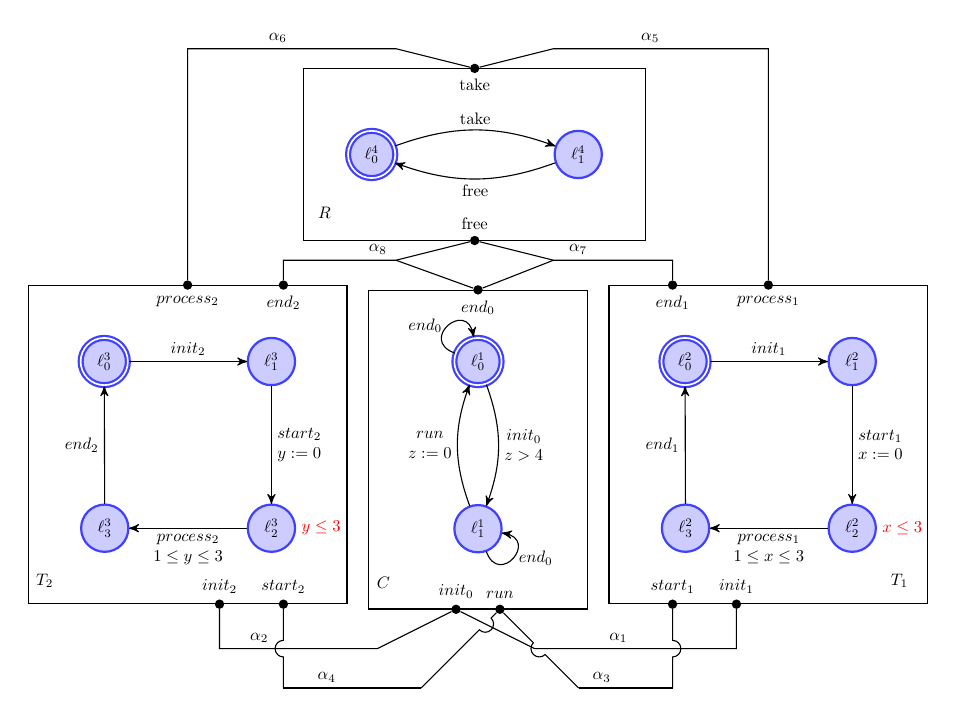
\begin{tikzpicture}[->,node distance=1.3cm,>=stealth',bend angle=20,auto,
  place/.style={circle,thick,draw=blue!75,fill=blue!20,minimum size=10mm},
  red place/.style={place,draw=red!75,fill=red!20}
  every label/.style={red},
  every node/.style={scale=.6},
  dots/.style={fill=black,circle,inner sep=2pt},
  initial text={}]

  \node [accepting, place] (l0)  {$\loc_0^1$};
  \node [place,below=1.5cm of l0,label={[shift={(-2,-1.9)}]$C$}] (l1) {$\loc_1^1$};

  \path (l0) edge [in=100, out=160,loop,looseness=4] node[left]{$end_0$} (l0)
         edge [bend left] node[right,align=center]{$init_0$\\$z>4$} (l1)
    (l1) edge [in=-10, out=-70,loop,looseness=4] node[right]{$end_0$} (l1)
         edge [bend left] node[left,align=center]{$run$\\$z:=0$} (l0);

  \node [accepting, place] (p1-0) [right=2cm of l0] {$\loc_0^2$};
  \node [place] (p1-1) [right=1.5cm of p1-0]{$\loc_1^2$};
  \node [place] (p1-2) [below=1.5cm of p1-1,label=right:\textcolor{red}{$x\le 3$},label={[shift={(1,-1.9)}]$T_1$}]            {$\loc_2^2$};
  \node [place] (p1-3) [left=1.5cm of p1-2] {$\loc_3^2$};

  \path (p1-0) edge node[align=center, pos=0.5]{$init_1$} (p1-1)
    (p1-1) edge node[align=center, pos=0.5]{$start_1$\\$x:=0$ } (p1-2)
    (p1-2) edge node[align=center, pos=0.5]{$process_1$ \\$1\le x\le3$ } (p1-3)
    (p1-3) edge node[align=center, pos=0.5]{$end_1$} (p1-0);


  \node [place] (p2-1) [left=2cm of l0]{$\loc_1^3$};
  \node [accepting, place] (p2-0) [left=1.5cm of p2-1]{$\loc_0^3$};
  \node [place] (p2-2) [below=1.5cm of p2-1,label=right:\textcolor{red}{$y\le 3$},label={[shift={(-4.8,-1.9)}]$T_2$}]            {$\loc_2^3$};
  \node [place] (p2-3) [left=1.5cm of p2-2] {$\loc_3^3$};

  \path (p2-0) edge node[align=center, pos=0.5]{$init_2$} (p2-1)
    (p2-1) edge node[align=center, pos=0.5]{$start_2$\\ $y:=0$ } (p2-2)
    (p2-2) edge node[align=center, pos=0.5]{$process_2$\\$1\le y\le3$ } (p2-3)
    (p2-3) edge node[align=center, pos=0.5]{$end_2$} (p2-0);

  \node [accepting, place] (r0) [above=2cm of l0,xshift=-2.25cm,label={[shift={(-1,-2)}]$R$}] {$\loc_0^4$};
  \node [place,right=2cm of r0] (r1) {$\loc_1^4$};

  \path (r0) edge [bend left] node[above]{take} (r1)
    (r1) edge [bend left] node[below]{free} (r0);

  \node [inner xsep=2cm,inner ysep=2cm,draw, yshift=-1mm, fit=(l0)(l1)] (rec1) {};
  \node [inner xsep=2cm,inner ysep=1.5cm,draw, fit=(r0)(r1)] (rec2) {};
  \node [inner xsep=2cm,inner ysep=2cm,draw, fit=(p1-0)(p1-1)(p1-2)(p1-3)] (rec3) {};
  \node [inner xsep=2cm,inner ysep=2cm,draw, fit=(p2-0)(p2-1)(p2-2)(p2-3)] (rec4) {};
%  \node [inner xsep=4cm,inner ysep=2.5cm,draw, fit=(rec1)(rec2)(rec3)(rec4)] (rec5) {};
 % \node [inner xsep=1.5cm,inner ysep=5mm,draw,above=5mm of rec1] (rec5) {

  %  $\begin{aligned}
  %    \gamma &=\{
  %  init_1=\{init,init_1\}, start_1=\{start,start_1\}, process_1=\{enter,proces_1\}, 
  %  end_1=\{end,exit,end_1\}, \\
   %  & init_2=\{init, init_2\}, start_2=\{start,start_2\}, 
   % process_2=\{enter,process_2\},end_2=\{end,exit,end_2\}\} 
  %  \end{aligned}$
 % };

  \node [dots,label=90:$init_2$] (i2) at ($(rec4.south west)!0.6!(rec4.south east)$) {};
  \node [dots,label=90:$start_2$] (s2) at ($(rec4.south west)!0.8!(rec4.south east)$) {};
  \node [dots,label=-90:$end_2$] (e2) at ($(rec4.north east)!0.2!(rec4.north west)$) {};
  \node [dots,label=-90:$process_2$] (p2) at ($(rec4.north east)!0.5!(rec4.north west)$) {};

  \node [dots,swap,label=90:$init_1$] (i1) at ($(rec3.south east)!0.6!(rec3.south west)$) {};
  \node [dots,swap,label=90:$start_1$] (s1) at ($(rec3.south east)!0.8!(rec3.south west)$) {};
  \node [dots,swap,label=-90:$end_1$] (e1) at ($(rec3.north west)!0.2!(rec3.north east)$) {};
  \node [dots,swap,label=-90:$process_1$] (p1) at ($(rec3.north west)!0.5!(rec3.north east)$) {};

  \node [dots,label=-90:take] (tr) at ($(rec2.north west)!0.5!(rec2.north east)$) {};
  \node [dots,label=90:free] (fr) at ($(rec2.south west)!0.5!(rec2.south east)$) {};

  \node [dots,label=90:$init_0$] (ic) at ($(rec1.south west)!0.4!(rec1.south east)$) {};
  \node [dots,label=90:$run$] (rc) at ($(rec1.south west)!0.6!(rec1.south east)$) {};
  \node [dots,label=-90:$end_0$] (ec) at ($(rec1.north west)!0.5!(rec1.north east)$) {};
  
  \path (tr) ++(0,0.25cm) +(-1cm,0) coordinate(xp2) +(1cm,0) coordinate(xp1);
  \draw  [-] (p1) |-node[above,xshift=-2.5cm]{$\alpha_5$} (xp1) -- (tr) -- (xp2)node[above,xshift=-2.5cm]{$\alpha_6$} -| (p2);

  \path (ic) ++(0,-0.5cm) +(1cm,0) coordinate(xi1) +(-1cm,0) coordinate(xi2);
  \draw[-,name path=line1] (i1) |-node[above,xshift=-2.5cm]{$\alpha_1$} (xi1) -- (ic) -- (xi2)node[above,xshift=-2.5cm]{$\alpha_2$} -| (i2); %here


  \path (rc) ++(0,-1cm) +(1cm,0) coordinate(sx1) +(-1cm,0) coordinate(sx2);

  \path[-,name path=line2] (s1) |-node[above,xshift=-1.5cm]{$\alpha_3$} (sx1) -- (rc) -- (sx2)node[above,xshift=-2cm]{$\alpha_4$} -| (s2); %here

 \path[name intersections={of=line1 and line2, by={a,b,c,d}}];% here

% draw semicircles at crossing points on the path
\coordinate (aux1) at (s2|-sx2);
\coordinate (aux2) at (s1|-sx1);
\draw[-,connect=(s2) to (aux1) over (d) by 3pt];
\draw[-] (aux1) -- (sx2);
\draw[-,connect=(sx2) to (rc) over (c) by 3pt];
\draw[-,connect=(rc) to (sx1) over (b) by 3pt];
\draw[-] (sx1) -- (aux2);
\draw[-,connect=(aux2) to (s1) over (a) by 3pt];

\path (fr) ++(0,-2.5mm) +(-1cm,0) coordinate(xe2) +(1cm,0) coordinate(xe1);
  \draw [-] (e1) |- node[above,xshift=-2cm]{$\alpha_7$}(xe1) -- (ec);
  \draw [-] (xe1) -- (fr);
  \draw [-] (e2) |- node[above,xshift=2cm]{$\alpha_8$}(xe2) -- (ec);
  \draw [-] (xe2) -- (fr);
% \path (i1) ++(-0.5cm,0) coordinate(xi1);
 % \path (i2) ++(0.2cm,0) coordinate(xi2);
 % \path (s1) ++(-0.2cm,0) coordinate(xs1);
 % \path (s2) ++(0.2cm,0) coordinate(xs2);
 % \path (e1) ++(-0.3cm,0) coordinate(xe1);
 % \path (e2) ++(0.3cm,0) coordinate(xe2);
 % \path (p1) ++(-0.2cm,0) coordinate(xp1);
 % \path (p2) ++(0.2cm,0) coordinate(xp2);
 % \draw  [-] (i1) -- (xi1) -- (ic);
 % \draw  [-] (i2) -- (xi2) -- (ic);
 % \draw  [-] (s1) -- (xs1) -- (rc);
 % \draw  [-] (s2) -- (xs2) -- (rc);
 % \draw  [-] (e2) -- (xe2) -- (ec);
 % %\draw  [-] (xe2) -- (fr);
 % \draw  [-] (e1) -- (xe1) -- (ec);
%  \draw  [-] (xe1) -- (fr);
\end{tikzpicture}
  \caption{Task Manager}
 \label{fig:run}
\end{figure*}  




\begin{example}[Running Example]
  \label{exp:run}
  Let us consider as a running example the composition of four components $C$, $T_1$, $T_2$, and $R$ of Figure~\ref{fig:run}.
  Component $C$ represents a  controller that initializes, releases, and ends tasks $T_1$ and $T_2$.
  Tasks use the shared resource $R$ during their execution.
  To implement such behavior, we consider the following interactions between $C$, $R$, and $T_1$: $\alpha_1=\{init_0, init_1\}$,
    $\alpha_3=\{run, start_1\}$, $\alpha_5=\{ take, process_1\}$, $\alpha_7 = \{end_0, free, end_1 \}$, 
      and similar interactions $\alpha_2$, $\alpha_4$, $\alpha_6$, $\alpha_8$ for task $T_2$, 
      as shown by connections on Figure~\ref{fig:run}.
      The controller is responsible for firing
      the execution of each task. First, it non-deterministically initializes one
      of the two tasks, i.e. executes $\alpha_1$ or $\alpha_2$, and then
      releases it through interaction $\alpha_3$ or $\alpha_4$.
      Tasks perform their processing independently of the controller, after being granted an access to the shared resource ($\alpha_5$ or $\alpha_6$).
      When ended by the controller, a task releases the resource  (interactions $\alpha_7$ or $\alpha_8$) and go back to its initial location.
      An example of execution sequence of the system of Figure~\ref{fig:run} is given below, in which valuations $v$ of clocks $x$, $y$, and $z$ are represented as a tuples $(\val(x),\val(y),\val(z))$:
      \begin{displaymath}
      %  \scriptsize{
        \small{
        \begin{split}
          &((\loc_0^1,\loc_0^2,\loc_0^3,\loc_0^4),(0,0,0))\transit{5}_{\gamma}((\loc_0^1,\loc_0^2,\loc_0^3,\loc_0^4),(5,5,5))\transit{\alpha_1}_{\gamma}((\loc_1^1,\loc_1^2,\loc_0^3,\loc_0^4),(5,5,5))\\
          &\transit{\alpha_3}_{\gamma}((\loc_0^1,\loc_2^2,\loc_0^3,\loc_0^4),(0,5,0))\transit{2}_{\gamma}((\loc_0^1,\loc_2^2,\loc_0^3,\loc_0^4),(2,7,2))\transit{\alpha_5}_{\gamma}
          ((\loc_0^1,\loc_3^2,\loc_0^3,\loc_1^4),(2,7,2))\\&\transit{3}_{\gamma}((\loc_0^1,\loc_3^2,\loc_0^3,\loc_1^4),(5,10,5))\transit{\alpha_2}_{\gamma}((\loc_1^1,\loc_3^2,\loc_1^3,\loc_1^4),
          (5,10,5))
        \end{split}
      }
      \end{displaymath}
    
\end{example}

\section{Local Planning of Interactions}
\label{sec3}
To the best of our knowledge, distributed platforms rarely offer built-in primitives
for the high level coordination, required by models where different components
need to synchronize together. Thus, the implementation of such models requires
an execution engine (for centralized execution), or more (for a more distributed execution),
responsible of coordinating components synchronizations using simpler primitives,
such as point-to-point messages passing (cite bip parrallel real time) and maybe a figure.

However, the semantics presented in previous section does not distinguish between 
an engine decision time and the actual execution time of components.
Particularly, communication delays induced by distributed platforms may introduce 
deadline misses during this process.
Additionally, Section~\ref{sec2} semantics is based on the global state of the system,
that is, the operational semantics rules is achieved through global states, which
break the principle of distribution where interaction execution should require only 
knowing the state of its participating components. 
We introduced in (cite FM) the \emph{weak planning semantics}, a semantics for local
planning of interaction within a defined upper bounded horizon. This semantics plans interaction based only on
the state of its involved components. This approach aim to differentiate the scheduling decision 
time of an interaction and its actual execution. In this paper we extend this work to lower bounded
horizons, which effectively, represent the estimation of the target platform communication
delays. In what follows, we first give some formal definitions, then we present our extension of
the weak planning semantics and discuss its properties.

\subsubsection*{Preliminaries}\label{subsec:wp}\mbox{}\\ 
We define the predicate $\plnIntxt{\alpha}{\delta}$ characterizing all states
  from which $\alpha$ can be planned and execute after $\delta$ units of time, that is, 
  $\alpha$ will be \emph{enabled} after a time progresses of $\delta$ units of time:
  \begin{equation}\label{eq:enf}
    \plnIn{\alpha}{\delta}
\end{equation}
%Notice that for $(\loc,\val),(\loc',\val')\in\reach(S)$, and $a_i\in\alpha$ we have:
%$$\enabledfrom(\alpha) \text{ at }(\loc,\val)\Rightarrow \enabled(\alpha) \text{ at } (\loc',\val'),\text{ such that }
%\loc_i=\loc'_i \text{ and } \val_i=\val'_i.$$

\begin{property}\label{pt:plnIn1}
  Let $(\loc,\val)$ be a state of the composition $S$. For any interaction $\beta\in\gamma$ such that, $\p{\alpha}\cap\p{\beta}=\emptyset$
  and $(\loc,\val)\transit{\beta}_{\gamma}(\loc',\val')$, where $\p{\alpha}$ (resp. $\p{\beta}$) represents components participating in 
  interaction $\alpha$ (resp. $\beta$), if $\plnIntxt{\alpha}{\delta}$ holds at state $(\loc,\val)$ then it still holds at state $(\loc',\val')$.
\end{property}
This property derives from the fact that executing interactions with disjoint set of components than $\alpha$ does not change the states
of components participating in $\alpha$, that is, for $a_i\in\alpha$ we have $\loc_i=\loc'_i$ and $\val_i=\val'_i$.


\begin{property}\label{pt:plnIn2}
  Let $(\loc,\val)$ and $(\loc,\val+\delta')$, with $\delta'\in\realpos$ be two states of the composition $S$. 
  If $\plnIntxt{\alpha}{\delta}$ is $\true$ at state $(\loc,\val)$ then $\plnIntxt{\alpha}{\delta-\delta'}$ is true at state
  $(\loc,\val+\delta')$ for $\delta'\le\delta$.
\end{property}
This property can be found directly by writing Equation~\ref{eq:enf} on state $(\loc,\val+\delta')$.

Let $\tcal{H}$ be a partial function $\tcal{H}: \gamma \to\realpos\times\realpos$ that defines for each
interaction $\alpha\in\gamma$, its respective planning horizons as an interval $[\hmn,\hmx]$. 
We define the predicate $\plntxt{\alpha}$ characterizing all states from which 
$\alpha$ can be planned w.r.t its planning horizons as follows:  
\begin{displaymath}
  \pln{\alpha}
\end{displaymath}
  with $\backhtxt$ represents an adaptation of the backward operators~\cite{tripakis98:thesis} that satisfies:
\begin{displaymath}
\backh
\end{displaymath}
\begin{property}\label{pt:pln}
  If the predicate $\plnIntxt{\alpha}{\delta}$ is $\true$ at a state $(\loc,\val)$, then the 
  predicate $\plntxt{\alpha}$ is also $\true$ for $\delta\in[\hmn,\hmx]$.
\end{property}

\begin{definition}[Plan]\label{def:plan}
We say that two interactions $\alpha$ and $\beta$, $\alpha \neq \beta$, \emph{conflicts} if $\p{\alpha}\cap\p{\beta}\neq\emptyset$, and we write $\alpha\#\beta$.
A plan $\pi$ is a partial function $\pi:\gamma \to\realpos$ defining relative times for 
executing a subset of non conflicting interactions, i.e.:
\begin{displaymath}
  \alpha\neq\alpha',\pi(\alpha)\neq\perp,\pi(\alpha')\neq\perp\implies \neg(\alpha\#\alpha').
\end{displaymath}
We also denote by $\confl(\pi)$ the set of interactions conflicting with the plan $\pi$, i.e. $\confl(\pi) = \{ \alpha \ | \ \exists \beta \# \alpha \ . \ \pi (\beta) \neq \bot \}$, and $\p{\pi}$ the set of components involved in interactions planned by $\pi$, i.e. $\p{\pi} = \{ B_i \ | \ \exists \alpha \ . \ \pi(\alpha) \neq \bot \wedge B_i \in \p{\alpha} \}$.
\end{definition}
%We write $(\alpha,\delta)\in\pi$ the planning of interaction $\alpha$ in $\delta$ units of 
We denote by $next \ \pi$ the closest relative execution time of interactions in the plan $\pi$, i.e. $next \ \pi = \textnormal{ min } \{ \pi(\alpha) \ | \ \alpha \in \gamma \wedge \pi(\alpha) \neq \bot \} \cup \{ +\infty \}$.
Notice that since $\pi$ stores relative times, whenever time progresses by $\delta$ the value $\pi(\alpha)$ assigned by $\pi$ to an interaction $\alpha$ should be decreased by $\delta$, until it reaches $0$ which means that $\alpha$ have to execute.
We write $\pi-\delta$ describing the progress of time 
over the plan, that is, $(\pi-\delta)(\alpha) = \pi(\alpha) - \delta$ for interactions $\alpha$ such that $\pi(\alpha) \neq \bot$.
We also write
$\pi-\alpha$ to denote the removal of interaction $\alpha$ from the plan $\pi$, i.e. $(\pi-\alpha)(\beta) = \pi(\beta)$ for any interaction $\beta \neq \alpha$, $(\pi-\alpha)(\alpha) = \bot$.
Similarly, $\pi \cup \{ \alpha \mapsto \delta \}$ assigns relative time $\delta$ to $\alpha$, $\alpha \notin conf(\pi)$, into existing plan $\pi$, i.e. $(\pi \cup \{ \alpha \mapsto \delta \})(\beta) = \delta$ for $\beta = \alpha$, $(\pi \cup \{ \alpha \mapsto \delta \})(\beta) = \pi(\beta)$ otherwise.
Finally, the plan $\pi$ such that $\pi(\alpha) = \bot$ for all interactions $\alpha \in \gamma$ is denoted by $\emptyset$.

We define below the semantics for planning each interaction $\alpha\in\gamma$ with $\delta$-horizon within $[\hmn,\hmx]$.

\begin{definition}[Planning Semantics]\label{def:pln_sem}
Given a set of components $\{B_1,\cdots,B_n\}$ and an interaction set $\gamma$,
we define the planning semantics of the composite component $S = (\Loc,\loc_0,\gamma,T_{\gamma},\X,\inv)$,
as the labeled transition system $S_p=(\Q_p,
\gamma\cup\realpos\cup\{\plana\},\tranbp{}{3})$ where:
\begin{itemize}
  \item $\Q_p=\Loc\times\mathcal{V}(\X)\times\Pi$, where $\Loc$ is the set of global location,
    $\mathcal{V}(\X)$ is the set of global clocks valuations, and $\Pi$ is the set of plans.
  \item $\plana$ defines the action of planning interactions
  \item $\tranbp{}{3}$ is the set of labeled transitions defined by the rules:
  \begin{itemize}
    \item Plan: $\alpha\in\gamma,\delta\in[\hmn,\hmx]$
    \begin{align*}
      &\hspace{4mm}\alpha\notin\confl(\pi)\wedge\plnIntxt{\alpha}{\delta}\\
     \cline{1-2}
     &(\loc,\val,\pi)\tranbp{\plan{\alpha,\delta}}{4}(\loc,\val,\pi\cup\{\alpha\mapsto\delta\}).\\
    \end{align*}
    \vspace*{-10mm}

    \item Exec: $\alpha\in\gamma$
     \begin{align*}
       &\hspace{14mm}\pi(\alpha)=0\\
            \cline{1-2}
          &(\loc,\val,\pi)\tranbp{\alpha}{3}(\loc',\val',\pi-\alpha)\}\\
        \end{align*}
  \item Time Progress: $\delta\in\realpos$
      \begin{align*}
        &\delta\le \text{next } \pi
        \wedge\tpc{i}(\val_i+\delta)_{i\in\{1,\cdots,n\}}\\
        \cline{1-2}
        &\hspace{4mm}(\loc,\val,\pi)\tranbp{\delta}{3}(\loc,\val+\delta,\pi-\delta)\\
          \end{align*}
  \end{itemize}
  \end{itemize}
\end{definition}
\begin{example}
  \label{exp:dl}
  Let us consider the following execution sequence for the example of Figure~\ref{fig:run} under the weak planning semantics rules and 
  for a value $\deltamax=5$ for all interactions except $\alpha_5$ and $\alpha_6$ that will be assigned a $\deltamax=3$:
      \begin{displaymath}
      %  \scriptsize{
        \small{
        \begin{split}
          &((\loc_0^1,\loc_0^2,\loc_0^3,\loc_0^4),(0,0,0),\emptyset)\tranbp{\plan{\alpha_1,5}}{6}((\loc_0^1,\loc_0^2,\loc_0^3,\loc_0^4),(0,0,0),\{\alpha_1\mapsto5\})\tranbp{5}{3}\\&
          ((\loc_0^1,\loc_0^2,\loc_0^3,\loc_0^4),(5,5,5),\{\alpha_1\mapsto0\})\tranbp{\alpha_1}{3}((\loc_1^1,\loc_1^2,\loc_0^3,\loc_0^4),(5,5,5),\emptyset)\tranbp{\plan{\alpha_3,2}}{6}
          \\&((\loc_1^1,\loc_1^2,\loc_0^3,\loc_0^4),(5,5,5),\{\alpha_3\mapsto2\})\tranbp{2}{3}((\loc_1^1,\loc_1^2,\loc_0^3,\loc_0^4),(7,7,7),\{\alpha_3\mapsto0\})\tranbp{\alpha_3}{3}
          \\&((\loc_0^1,\loc_2^2,\loc_0^3,\loc_0^4),(0,7,0),\emptyset)\tranbp{\plan{\alpha_5,2}}{6}((\loc_0^1,\loc_2^2,\loc_0^3,\loc_0^4),(0,7,0),\{\alpha_5\mapsto2\})\tranbp{2}{3}
          \\&((\loc_0^1,\loc_2^2,\loc_0^3,\loc_0^4),(2,9,2),\{\alpha_5\mapsto0\})\tranbp{\alpha_5}{3}((\loc_0^1,\loc_3^2,\loc_0^3,\loc_1^4),(2,9,2),\emptyset)\tranbp{\plan{\alpha_2,3}}{6}\\
            &((\loc_0^1,\loc_3^2,\loc_0^3,\loc_1^4),(2,9,2),\{\alpha_2\mapsto3\})\tranbp{3}{3}((\loc_0^1,\loc_3^2,\loc_0^3,\loc_1^4),(5,12,5),\{\alpha_2\mapsto0\})\tranbp{\alpha_2}{3}\\
            &((\loc_1^1,\loc_3^2,\loc_1^3,\loc_1^4),(5,12,5),\emptyset)\tranbp{\plan{\alpha_4,0}}{6}((\loc_1^1,\loc_3^2,\loc_1^3,\loc_1^4),(5,12,5)\{\alpha_4\mapsto0\})\tranbp{\alpha_4}{3}\\
            &((\loc_0^1,\loc_3^2,\loc_2^3,\loc_1^4),(5,0,0),\emptyset)\tranbp{\plan{\alpha_7,4}}{6}((\loc_0^1,\loc_3^2,\loc_2^3,\loc_1^4),(5,0,0),\{\alpha_7\mapsto4\})\tranbp{3}{3}\\
            &((\loc_0^1,\loc_3^2,\loc_2^3,\loc_1^4),(8,3,3),\{\alpha_7\mapsto1\})
        \end{split}
      }
      \end{displaymath}
This execution sequence represents a path that alternates plan actions, time steps and execution of some interactions. We can see that for interaction
$\alpha_7$ which is planned 4 units of time ahead, the system cannot reach the state from which it can be executed since there is a time progress expiration
in component $T_2$ after 3 time units from planning this interaction. This means that local planning of interactions doesn't always allow the progress of time and may
thus, introduce deadlocks even if the system under the global semantics rules is deadlock-free. 
      
\end{example}

\subsection{Relation between Global and Weak Planning Semantics}
We use weak simulation to compare the model under
the global state semantics rules and the one under the planning semantics rules
by considering \plana-transitions unobservable.
As explained in Example~\ref{exp:dl}, the planning semantics does not preserve the deadlock freedom property of our system.
Nevertheless, the following proves weak simulation relations between the two semantics.

\begin{theorem}\label{thm:pi_pln}
  For all the reachable states $(\loc,\val,\pi)$ of the planning semantics, and $\forall\alpha\in\pi$, the
  predicate $\plnIntxt{\alpha}{\pi(\alpha)}$ is $\true$.
\end{theorem}

Let $S_g=(\Q_g,\gamma\cup\realpos,\transit{}_{\gamma})$ (resp. $S_{p}=(\Q_{p},\gamma\cup\realpos\cup\{\plana\},\tranbp{}{3})$)
the labeled transition system characterizing the global (resp. planning) semantics. 
\begin{proposition}\mbox{}\\
  \label{prop:relation}
  \vspace{-6mm}
  \begin{description}[labelwidth=1.5cm]
    \item[\namedlabel{itm:1}{Relation 1}]$\forall\delta\in\realpos.(\loc,\val,\pi)\tranbp{\delta}{3}(\loc',\val',\pi')
      \Rightarrow (\loc,\val)\transit{\delta}_{\gamma}(\loc',\val')$
    \item[\namedlabel{itm:2}{Relation 2}]$\forall\alpha\in\gamma.(\loc,\val,\pi)\tranbp{\alpha}{3}(\loc',\val',\pi')
      \Rightarrow (\loc,\val)\transit{\alpha}_{\gamma}(\loc',\val')$
  \end{description}
\end{proposition}
It is straightforward that~\ref{itm:1} is a consequence of the definition of time progress in the planning semantics. For Relation~\ref{itm:2},  
using Definition~\ref{def:plan}, we can deduce that:\\
\begin{displaymath}
(\loc,\val,\pi)\tranbp{\alpha}{3}(\loc',\val',\pi')\Rightarrow \pi(\alpha)=0,
\end{displaymath}
By Theorem~\ref{thm:pi_pln}, this implies that $\plnIntxt{\alpha}{0}$ is $\true$ at state $(\loc,\val,\pi)$, meaning that $\enabled(\alpha)$ is
also $\true$, which allows to infer~\ref{itm:2}.  

\begin{corollary}\label{cr:reach}
  If a state $(\loc,\val,\pi)\in\reach(S_p)$, then $(\loc,\val)\in\reach(S_g)$.
\end{corollary}

\begin{definition}[Weak Simulation]
  A weak simulation over $A=(\Q_A,\sum\cup\{\beta\},\to_A)$ and $B=(\Q_B,\sum\cup\{\beta\},
  \to_B)$ is a relation $R\subseteq \Q_A\times \Q_B$ such that we have: 
  $\forall(q,r)\in R, a\in \sum .q\transit{a}_A q' \implies\exists r':(q',r')\in R\wedge r\transit{
  \beta^*a\beta^*}_B r' \text{ and } \forall(q,r)\in R: q\transit{\beta}_Aq'\implies\exists r':
  (q',r')\in R\wedge r\transit{\beta^*}r'$.
  B simulates A, denoted by $A\simu{R}B$, means that B can do everything A does.
\end{definition}
The definition of weak simulation is based on the unobservability of $\beta-$transitions. In our case, $\beta-$transitions corresponds to $\plana-$transitions.
\begin{corollary}\label{cr:sim}
  $S_p\simu{R_1} S_g$ with $R_1=\{(\q,\pi);\q)\in\Q_p\times\Q_g\}$.
\end{corollary}

Corollary~\ref{cr:sim} corresponds to a notion of correctness of the planning semantics: any execution in the planning semantics corresponds to an execution in the global state semantics.

By contrast to (cite fm), where planning immediately, i.e. with a zero horizon, was allowed, 
by introducing a minimal horizon of planning interactions, the planning semantics does no longer
preserve all execution sequences of the global state semantics.

As explained in example, the planning semantics may introduce deadlocks as shown by the scenario presented in Example~\ref{exp:dl}.
In the following, we present different verification methods to check the deadlock freedom of a system under the planning semantics rules.






\section{Planning Semantics Correctness}
\label{sec4}
Local planning of interactions consists effectively in applying a local time step, followed
by the execution of an interaction. Even if local time steps are allowed in planned components,
it may be disallowed in the rest of the system. Additionally, planning horizons 
insert a certain latency between interactions, which can result in missing interactions deadlines in some cases.
Thus, as explained in Example, the planning semantics may 
exhibit deadlock situations nonexistent in the system under the global state semantics, since:
\emph{(i)} it does not consider time progress conditions of components not participating in 
planned interactions, and \emph{(ii)} it introduces a certain latency between interaction executions. 

Since the application model does not consider delays between interactions,
in case of urgency of a time progress condition, semantically, consecutive executions can happen
in the global state semantics and enable thus to get ride of this urgency. Thing that does not hold in the planning semantics.
In what follows, we present different methodologies in order to enforce system correctness under
the planning semantics rules. 

\subsubsection{Planning Semantics Restriction}\mbox{}\\
\label{sec4:1}
For the sake of simplicity, we assume that all interactions have the same lower bound  
planning horizon, that is, $\forall\alpha,\beta\in\gamma$ such that $\alpha\neq\beta$,
$\hmn=\hmnb{\beta}=h_{\min}$.
In order to enforce the correctness of the planning semantics, we restrict the condition
of time progress as follows:
\begin{equation}
\label{eq:tpc_rest}
\begin{split}
  &\delta\le \text{next } \pi
  \wedge\forall B_i\notin\p{\pi}.\tpc{i}(\val_i+\delta+h_{\min})\\
  %\urg(\tpc{\loc_i}(\val_i+\delta+\delta'))\forall\delta'<h_{\min}\\
        \cline{1-2}
        &\hspace{12mm}(\loc,\val,\pi)\tranbp{\delta}{3}(\loc,\val+\delta,\pi-\delta)\\
\end{split}
\end{equation}
This restriction aims to disallow any time progress, if there is a component not
participating in any interaction of the plan such that it progresses out of its
allowed planning intervals.

Let $\dot{S_{p}}=(\Q_{p},\gamma\cup\realpos\cup\{\plana\},\tranbp{}{3})$
the labeled transition system characterizing the planning semantics under
the restriction~\ref{eq:tpc_rest}. 

\begin{corollary}\label{cr:sim2}
  $\dot{S_p}\simu{R_1} S_g$ with $R_1=\{(\q,\pi);\q)\in\Q_p\times\Q_g\}$.
\end{corollary}

\subsubsection{Deadlock Characterization}

%\begin{theorem}[Local Deadlock]
%  \label{thm:local_dl}
%  Let $\{B_1,\cdots,B_n\}$ be a set of components and $\gamma$ an interaction set. 
%  Let $\loc_i\in\Loc_i$ be a location of a component $B_{i\in\{1,\cdots,n\}}$ 
%  such that $\tpc{\loc_i}\neq\true$. Let $\Gamma(\loc_i)$ be the subset of interactions
%  including all actions possible from the location $\loc_i$, that is,
%  $\Gamma(\loc_i)=\{\alpha|\exists\loc_i\transit{a_i,g_i,r_i}\loc'_i.a_i\in\alpha\}$.
%  If it exists a reachable state $(\loc,\val,\pi)$ of the planing semantics 
%  such that: 
%  \[\exists\loc_i\in\loc,\val_i=\tpc{\loc_i-h_{\min}}.\forall\alpha\in\Gamma\ \neg\plntxt{\alpha}\] 
%  then component the $B_i$ locally deadlocks under the planning semantics rules, and thus, the composition under 
%  the planning semantics rules deadlocks.
%\end{theorem}

%Condition of Theorem~\ref{thm:local_dl} enables to identifies models where the time progress condition
%of a component is affected by the execution of interactions including other components.

\begin{theorem}
  \label{thm:dl}
  If a reachable state $(\loc,\val,\pi)$ of the composition $S=\gamma(B_1,\cdots,B_n)$ under
  the planning semantics rules deadlocks, then the following is satisfied:
  \begin{adjustwidth}{-10mm}{-10mm}
  \begin{equation}\label{eq:dl}
  \begin{split}
    &\bigvee_{B_i\in S\setminus\p{\pi}}\Big[\Big(
    \underbrace{\bigvee_{\loc_i\in\Loc_i}\at{\loc_i}
  \wedge\urg(\tpc{\loc_i}(\val_i+h_{\min}))\Big)}_\text{\mytag{A}{A}}\wedge
    \Big(\underbrace{\bigwedge_{\alpha\in\Gamma(B_i)\setminus\confl(\pi)}\hspace{-8mm}
    \neg\plntxt{\alpha}\vee\hspace{-5mm}\bigvee_{\alpha\in\Gamma(B_i)\cap\confl(\pi)}
\hspace{-8mm}\plntxt{\alpha}}_\text{\mytag{B}{B}}\Big)\Big]\\
&\hspace{4.5cm}\wedge\underbrace{\bigwedge_{\alpha\in\pi}\Big(\pi(\alpha)\neq0\wedge
    \plnIntxt{\alpha}{\pi(\alpha)}\Big)}_\text{\mytag{C}{C}} 
  \end{split}
  \end{equation}
  \end{adjustwidth}
\end{theorem}

Theorem~\ref{thm:dl} characterizes deadlock states of the planning semantics. Precisely,
terms A of Equation~\ref{eq:dl} represents the time progress restriction as presented
in~\ref{eq:tpc_rest}. It expresses clocks valuations, in a component not participating 
in the planned interaction, $h_{\min}$ units of time before its expiration. On the other hand,
term B describes the cause of the time progress restriction, that is, all interactions
of $\Gamma(\loc_i)$ are not plannable either because (1) they are conflicting with the plan
or, (2) because they are not in their corresponding planning states.
Finally, term C depicts the existence of interactions in the plan and the fact that none of them
reached yet their execution dates.
 
\begin{theorem}\label{thm:dla}
  Let $\phi(\alpha)$ be the following predicate:

  \begin{adjustwidth}{-10mm}{-10mm}
    \begin{equation}\label{eq:dla}
  \begin{split}
    &\bigvee_{B_i\in S\setminus\p{\alpha}}\Big[\Big(
    \bigvee_{\loc_i\in\Loc_i}\at{\loc_i}
  \wedge\urg(\tpc{\loc_i}(\val_i+h_{\min}))\Big)\wedge
    \Big(\bigwedge_{\beta\in\Gamma(B_i)\setminus\confl(\alpha)}\hspace{-8mm}
    \neg\plntxt{\beta}\vee\hspace{-5mm}\bigvee_{\beta\in\Gamma(B_i)\cap\confl(\alpha)}
\hspace{-8mm}\plntxt{\beta}\Big)\Big]\\
&\hspace{6.5cm}\wedge\tilde{\plntxt{\alpha}} 
  \end{split}
\end{equation}
  \end{adjustwidth}
  where $\tilde{\plntxt{\alpha}}$ is the obtained predicate by replacing 
  $h_{\min}$ by 0 in $\plntxt{\alpha}$ and transforming the upper 
  timing constraints of interaction $\alpha$ to strict guards.
  If a reachable state $(\loc,\val,\pi)$ deadlocks then $\exists\alpha\in\gamma$ 
  such that $\phi(\alpha)$ is satisfied.
\end{theorem}

Since reachable states of the restricted planning semantics are reachable 
in the global state semantics (Corollary~\ref{cr:sim2}), we can deduce that if for
every interaction of $\gamma$, Equation~\ref{eq:dla} is unsatisfied, then the system
under the restricted planning semantics is deadlock-free.



\section{Appendix}

\begin{proof}[Theorem~\ref{thm:dla}]
  Let $(\loc,\val,\pi)$ be a reachable deadlock state of the planning semantics. This 
  means that Equation~\ref{eq:dl} is satisfied, meaning that $\exists\alpha\in\pi$ 
  satisfying:
  \begin{equation}\label{1}
    \Big(\bigwedge_{\beta\in\Gamma(B_i)\setminus\confl(\alpha)}\hspace{-8mm}
    \neg\plntxt{\beta}\vee\hspace{-5mm}\bigvee_{\beta\in\Gamma(B_i)\cap\confl(\alpha)}
    \hspace{-8mm}\plntxt{\beta}\Big)\wedge\pi(\alpha)\neq0\wedge
    \plnIntxt{\alpha}{\pi(\alpha)}
  \end{equation}
  We have:
  \begin{align}
  \pi(\alpha)\neq0\wedge\plnIntxt{\alpha}{\pi(\alpha)}
  &\Rightarrow\tilde{\plntxt{\alpha}}\label{2}\\
  \bigvee_{B_i\in S\setminus\p{\pi}}\bigvee_{\loc_i\in\Loc_i}\at{\loc_i}\wedge\urg(\tpc{\loc_i}(\val+h_{\min}))&\Rightarrow\bigvee_{B_i\in S\setminus\p{\alpha}}\bigvee_{\loc_i\in\Loc_i}\at{\loc_i}\wedge\urg(\tpc{\loc_i}(\val+h_{\min})\label{3}
   \end{align}
     
   By combining~\ref{1},~\ref{2} and~\ref{3} we obtain Equation~\ref{eq:dla}, which
   proves Theorem~\ref{thm:dla}


\end{proof}



\bibliographystyle{abbrv} 
\bibliography{main}
\end{document}
